\documentclass[titlepage]{article}

\usepackage{./estilos/estiloBase} % Basicamente son todas las
                                  % librerias usadas. En caso de que
                                  % falten librerias se van añadiendo
                                  % al fichero.
\usepackage{./estilos/colores}  % Algunos colores ya generados, para
                                % los algunos estilos más avanzados.
\usepackage{./estilos/comandos} % Algunos comandos personalizados

\setlength{\unitlength}{1 cm} %Especificar unidad de trabajo

\begin{document}

% ------- %
% PORTADA %
% ------- %

\thispagestyle{empty}
\begin{picture}(0,0)
\put(-0.3,-3){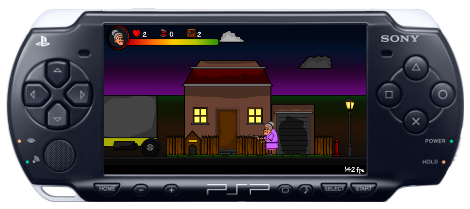
\includegraphics[scale=0.7]{portpsp.png}}
\end{picture}\\[4cm]

\begin{center}
\textbf{{\Huge Desarrollo de videojuegos para PSP con C++ y SDL}}\\[5cm]
{\large David Saltares Márquez}\\[5cm]
Este documento posee una licencia \href{http://creativecommons.org/licenses/by-sa/3.0/es/}{Creative Commons (by-sa)}\\[1cm]

\includegraphics[scale=1]{cc.png}
\end{center}
\clearpage

\tableofcontents
\clearpage

\section{Introducción}
Bienvenido al manual de \emph{Granny's Bloodbath}, si estás leyendo esto es que estás mínimamente interesado en lo que hemos hecho lo que nos honra enormemente. \emph{Granny's Bloodbath} es un juego de plataformas y acción protagonizado por una abuelita. Ha sido desarrollado para la asignatura de Diseño de Videojuegos en la Universidad de Cádiz en C++ utilizando la librería SDL. Te deseamos que lo pases lo mejor posible y que aniquiles a todos los zombies que puedas, ¡salva a la abuelita!\\

A lo largo del manual verás los requisitos mínimos, una brevísima guía de instalación, los detalles de la historia y sus personajes así como los controles básicos. A continuación, la sección más interesante de este manual: \textbf{crear tus propios niveles para el juego}. Sería genial que colaboraras con la comunidad y aportaras tu granito de arena a nuestro trabajo.\\

\emph{Granny's Bloodbath} es Software Libre y se distribuye bajo una licencia GPL. Básicamente puedes distribuirlo con toda libertad así como consultar su código fuente o modificarlo. Para más detalles sobre la licencia GPL puedes consultar el anexo correspondiente.\\

¡Que disfrutes!


\section{Instalación}
Descargar e instalar \emph{Granny's Bloodbath} es de lo más sencillo, a continuación explicamos el proceso.

\begin{itemize}
	\item Entra en la sección de descargas del blog oficial:\\
		\href{http://grannysbloodbath.wordpress.com/descargas/}{http://grannysbloodbath.wordpress.com/descargas/}
	\item Elije la última versión disponible acorde con tu sistema operativo y descárgala
	\item Según tu sistema deberás realizar uno de los siguientes pasos:
\end{itemize}

\subsection{Instalación en Windows}
Descomprime el fichero obtenido en el directorio deseado y... ¡Listo, ya puedes jugar!\\

Puede que en un futuro creemos un setup que permita elegir directorio de instalación así como creación de accesos directos. No obstante, por el momento creemos que así es suficiente. Cuanto más sencillo mejor, ¿no?

\subsection{Instalación en GNU/Linux}
Descomprime el fichero obtenido en el directorio deseado.\\

Debes tener instalados los paquetes: libsdl, libsdl-mixer, libsdl-image, libsdl-ttf. Si no los tienes abre una terminal y escribe:

\lstinputlisting[style=consola]{paquetes.sh}

Es probable que no puedas ejecutar el juego por problemas con los permisos, si ese es tu caso debes de hacer lo siguiente en la terminal:

\lstinputlisting[style=consola]{permisos.sh}

Vale, ha sido un proceso un poco más largo pero... ¡Ya puedes jugar! Puede que más adelante creemos un paquete \emph{.deb} para que la instalación sea mucho más sencilla.


\section{El makefile}
El makefile para compilar proyectos para PSP tiene ciertas particularidades
dignas de mención en esta humilde guía.\\

Vamos a suponer que tenemos la siguiente jerarquía de directorios:

\begin{verbatim}
|- Proyecto
    |- makefile
    |- main.cpp
    |- engine
       |- ficheros.cpp
       |- ficheros.h
\end{verbatim}

Nuestro makefile sería algo similar a lo siguiente:

\lstinputlisting[style = consola]{makefile.txt}

Podemos personalizar la apariencia de nuestro $homebrew$ en el menú de PSP
mediante las siguientes variables:

\begin{itemize}
	\item \textbf{PSP\_EBOOT\_ICON}: icono de 144x80 que identificara al
	juego en la sección $Juegos$ del menú.
	\item \textbf{PSP\_EBOOT\_PIC1}: fondo que aparecerá en la consola cuando
	el juego esté seleccionado, debe tener 480x272.
	\item \textbf{PSP\_EBOOT\_SND0}: fichero de sonido en formato at3
	que se escuchará cuando nuestro juego esté seleccionado en el menú.
\end{itemize}


\section{Callbacks de salida al SO}
Seguramente sabréis de qué hablo pero es probable que no os hayáis dado
cuenta de que debe ser algo a controlar a la hora de portar la aplicación
a PSP. Me refiero a la pausa del juego y a la vuelta al sistema operativo
de la consola. En cualquier momento podemos pulsar el botón $HOME$, seleccionar
`salir del juego' y volver al menú principal. Si no tenemos cuidado
provocaremos un cuelgue en la consola cada vez que queramos salir.\\

Tendremos que definir ciertas funciones que actúen como $callbacks$. Un fichero
$main.cpp$ de un port génerico podría ser el siguiente:

\lstinputlisting[style = C++]{main.cpp}

Es importante comprender que cuando el usuario decide salir del juego
(esperemos que no sea demasiado a menudo) se llama a la función
$exit\_callback$ por lo que debe ser ella la que se encargue de hacer
los cambios pertinentes para romper el game-loop. En mi caso una forma
podía ser llamar a la al método $set\_quit()$ de mi clase $keyboard$ pero
en el vuestro puede ser cualquier otro.


\section{La pantalla}
Las dimensiones de la pantalla de la PSP son de 480x272 píxeles por lo que
la superficie principal de SDL a crear debe ser exactamente de dichas dimensiones.
Por otro lado está la profundidad de color, inicialmente pensé que sería más
eficiente bajar dichos niveles de 32bpp a 16bpp o incluso 8bpp si fuera necesario
por cuestiones de rendimiento. No obstante, el port de SDL para PSP
parece no funcionar correctamente en los dos últimos modos. Finalmente acabé
usando 32bpp aunque el rendimiento final es bastante bueno.\\

La llamada para inicializar SDL en PSP puede ser algo similar a esto:

\lstinputlisting[style = C++]{inicializar.cpp}

Con las correspondientes comprobaciones posteriores.


\section{Leyendo la entrada de PSP}
Teóricamente, como la mayoría de tutoriales apuntan, podemos usar
$SDL\_Joystick$ para manejar la entrada del jugador. Se nos presenta una equivalencia
entre botones de joystick y de PSP para que podamos manejarla pero lo cierto
es que, o soy tremendamente torpe, o este sistema no funciona del todo bien.\\

Finalmente, para $Granny's bloodbath$ decidí cambiar la implementación 
de la clase que manejaba la entrada del jugador (utilizando la API de las librerías de PSP) 
sin cambiar su interfaz, de ese modo me adaptaba a las circunstancias de PSP sin
afectar al resto del sistema.\\

Las clases que utilicé son las siguientes y funcionan bastante bien:\\

\textbf{keyboard.h}:

\lstinputlisting[style = C++]{keyboard.h}

\textbf{keyboard.cpp}:

\lstinputlisting[style = C++]{keyboard.cpp}



\section{Conclusiones}
\input{conclusiones.tex}

\end{document}
